\documentclass[a4]{article}
\usepackage[utf8]{inputenc}
\usepackage{amssymb}
\usepackage{graphicx}
\usepackage{caption}
\usepackage[french]{babel}
\author{Clément Caumes}
\title{Premier TD MI100}
\date{\today}

\begin{document}
\maketitle
\section{Introduction}
\section{Enoncés des exercices}
\subsection{Poker}
\begin{enumerate}
\item Combien de \textbf{mains} de 5 cartes sont possibles avec {\tiny un jeu} de 52 cartes ?
\item Combien avec 2 as {\huge exactement} ? 
\end{enumerate}
\subsection{Si vous répondez mal, gare...}
Un père {\large logicien} dit à son fils \textsf{fais tes devoirs ou je te colle une baffe.} (voir \ref{figure 1}) Le fils se dépêche de faire ses devoirs et retourne 
annoncer à son père qu'il les a fini. Celui-ci lui dit c'est très bien et \texttt{lui colle une baffe.} \textit{Le père est il cohérent avec ses déclarations?}
\textbf{Approuvez-vous ses méthodes pédagogiques ?}
\subsection{Tables de vérités}
Ecrire les tables de vérité de $A \Rightarrow B$ et de $\urcorner B\Rightarrow \urcorner A$. Que constatez-vous ? 
\section{Correction des exercices}
\subsection{Poker}
\begin{itemize}
\item Le nombre de mains de 5 cartes au poker vaut : 
\[C^{5}_{52}= \frac{52!}{(52-5)!5!}=\frac{52 \times 51 \times 50 \times 49 \times 48}{5!}=2.59896 \times 10^{6}\]
\item Le nombre de mains de poker avec exactement 2 as vaut :
\[C^{2}_{4} \times C^{3}_{48}= \frac{4!}{2!2!} \times \frac{48!}{45!3!} =103776\]
\end{itemize}
\begin{figure}[h]
\subsection{Si vous répondez mal, gare...}
Voici une représentaion du père logicien :\\
\centering
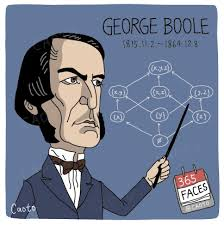
\includegraphics[scale=0.5]{boole.jpg}
\label{figure 1}
\caption{Representation du père booléen}
\end{figure}
\subsection{Tables de vérités}
La table de vérité de $A \urcorner B$ est la suivante :
\vspace {0,5cm}

\begin{tabular}[h]{|c|c||c|}
\hline
A & B & $A \Rightarrow B$\\
\hline
\hline
0 & 0 & 1\\
\hline
0 & 1 & 1\\
\hline
1 & 0 & 0\\
\hline
1 & 1 & 1\\
\hline
\end{tabular}
\vspace{0,5cm}

La table de vérité de $\urcorner B \Rightarrow \urcorner A$ est la suivante :\\

\begin{tabular}[h]{|c|c||c|c||c|}
\hline
A & B & $\urcorner B$ & $\urcorner A$ & $\urcorner B \Rightarrow \urcorner A$ \\
\hline
0 & 0 & 1 & 1 & 1\\
\hline
0 & 1 & 1 & 0 & 1\\
\hline
1 & 0 & 0 & 1 & 0\\
\hline
1 & 1 & 0 & 0 & 1\\
\hline
\end{tabular}

\section{Conclusion}
\end{document}
